\section{Physical Layer}
\paragraph{Schicht 1: Bitübertragungsschicht}
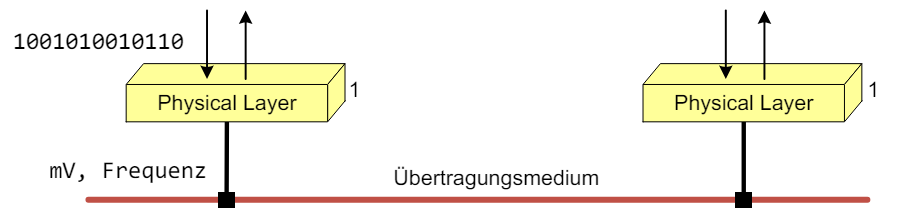
\includegraphics[width=0.75\linewidth]{images/Physical_Layer.png}

\begin{definition}{Funktionalität}
    ungesicherte Übertragung eines Bit-Stroms
\begin{itemize}
    \item Elektrische Eigenschaften (Signalform, Amplituden, etc.)
    \item Codierung (Abbildung der Daten auf elektrische Signale)
    \item Mechanische Eigenschaften (Stecker, Pinbelegung etc.)
\end{itemize}
\end{definition}

\subsubsection{Verkehrsbeziehung und Kopplung}
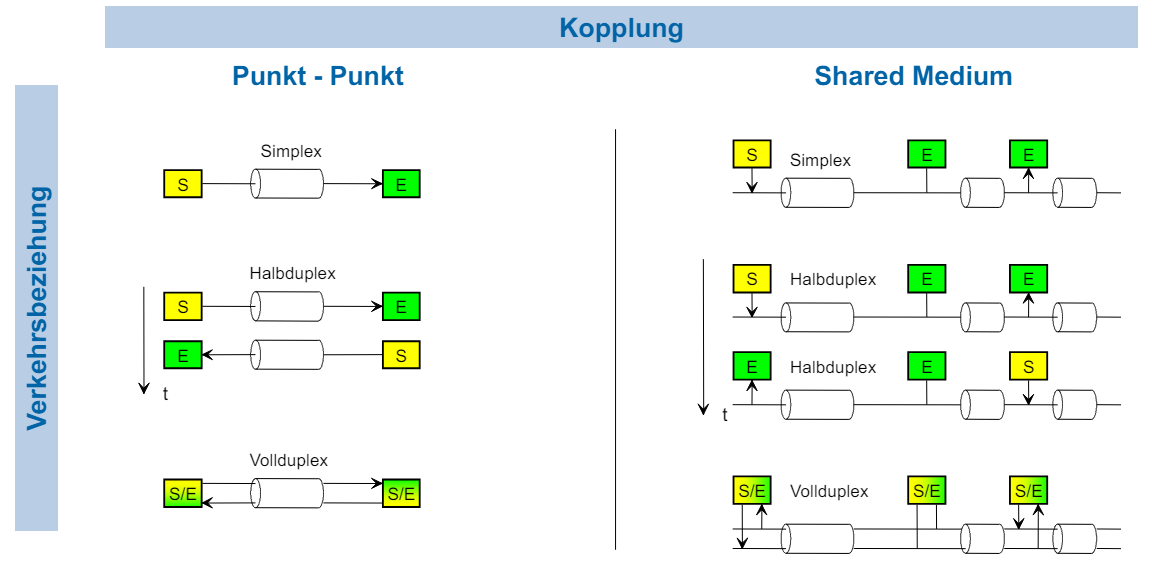
\includegraphics[width=1\linewidth]{images/Verkehrsbeziehung_Kopplung.png}

\begin{concept}{Arten der Kommunikation (Verkehrsbeziehung) und Kopplung}
    \begin{itemize}
        \item Simplex: Ein Kanal, eine Richtung
        \item Halbduplex: Ein Kanal, abwechslungsweise in 2 Richtungen
        \item Vollduplex: Ein Kanal pro Richtung
        \item Punkt-Punkt: Direkte Verbindung 2 Kommunikationspartnern
        \item Shared Medium: Mehrere Partner verwenden das gleiche Medium
    \end{itemize}
\end{concept}

\subsubsection*{Einheiten und Kenngrössen}

\begin{KR}{Wichtige Kenngrössen}
    \begin{itemize}
        \item Bandbreite B – Einheit Hertz (Hz)
        \begin{itemize}
            \item Maximal übertragbare Frequenz, durch Medium limitiert
        \end{itemize}
        \item Symbolrate $f_s$ – Einheit Baud (Bd)
        \begin{itemize}
            \item \# Symbole pro Zeit, limitiert durch Bandbreite ($\leq$ 2B)
        \end{itemize}
        \item Bitrate R – Einheit Bit/s (bps)
        \begin{itemize}
            \item R = Symbolrate $\times$ Anzahl Bits pro Symbol
        \end{itemize}
        \item Kanalkapazität C – Einheit Bit/s (bps)
        \begin{itemize}
            \item Berücksichtigt realen Kanal SNR $\frac{S}{N}$
        \end{itemize}
    \end{itemize}
\end{KR}

\begin{remark}
    Bitrate nominell gleich wie Symbolrate wenn: Informationsgehalt pro Symbol = 1 Bit $\rightarrow$
    z.B. bei binärer Codierung (2 Zustände)
\end{remark}

\begin{remark}
    \begin{itemize}
        \item In der Kommunikation stehen k, M, G etc. SI-konform für die exakten Zehnerpotenzen:
        \begin{itemize}
            \item kBit = $10^3$ Bit, MBit = $10^6$ Bit, GBit = $10^9$ Bit
        \end{itemize}
        \item Bitrate/Datenübertragungsrate/Durchsatz = Synonyme
        \item Bandbreite = maximale Symbolrate
    \end{itemize}
\end{remark}

\begin{remark}
    ld = log2, lg = log10, ln = natürlicher Logarithmus
\end{remark}

\subsubsection{Datenrate, Bandbreite, Bandrate}

\begin{formula}{Datenübertragungsrate} $f_s \leq 2B$
\end{formula}

\begin{formula}{Maximal erreichbare Bitrate} $R[bit/s] = R \leq 2B \cdot log_2(M)$
    \vspace*{1mm}\\
    Unterscheidbare Signalzustände:
    $M = 1 + \frac{A}{\Delta V}$
\end{formula}
\begin{remark}
    A = Max. Grösse Signals,
    V = Ungenauigkeit Empfänger
\end{remark}

\centering
    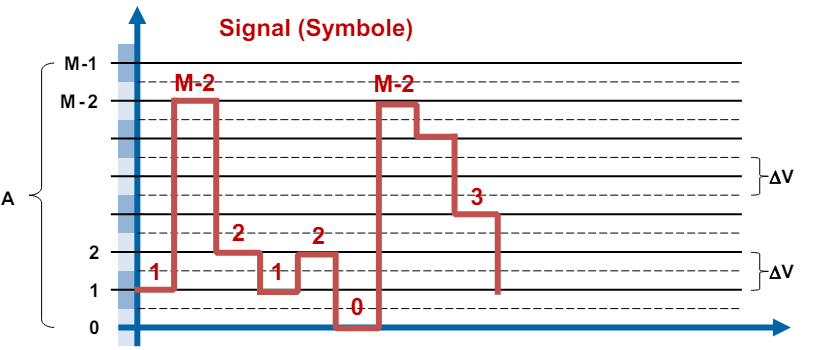
\includegraphics[width=0.8\linewidth]{images/max_bitrate_actual.png}

\begin{formula}{Kanalkapazität}
    $C_s = B \cdot log_2(1 + \frac{S}{N})$
\end{formula}

\begin{remark}
    S: Signalleistung,
    N: Rauschleistung
\end{remark}

\subsubsection{Übertragungsverfahren: Parallel und Seriell}

\begin{definition}{Serielle asynchron Übertragung}\\
    Benötigte Abmachungen zwischen Sender und Empfänger:
    \begin{itemize}
        \item Bitrate, \# Datenbits (typ. 1 Byte), \# Stoppbits (typ. 1 Bit)
        \item Parität (gerade, ungerade, keine)
    \end{itemize}
    Taktrückgewinnung möglich
\end{definition}

\begin{example}
    \includegraphics[width=1\linewidth]{images/serielle_asynchrone_übertragung.png}
    \begin{itemize}
        \item Empfangen wird 1001 1100 – LSB first –> 0011 1001 (binär); 0x39 (hex); ASCII Code 57 = «9»
    \end{itemize}
    Genauigkeitsanforderung an Takte von Sender und Empfänger:
    \begin{itemize}
        \item Letzte Abtastung muss noch im Zeitfenster liegen (Stop-Bit bei einem Stop-Bit); also ½T auf 9½ T
    \end{itemize}
\end{example}

\begin{KR}{Clock Drift}\\
    Maximale Framegrösse Ethernet: 1’500 Bytes.
    \begin{itemize}
        \item Standard: Oszillatoren brauchen Genauigkeit von ±50 ppm 
        \item 50 ppm (parts per million) $\rightarrow$ Fehler von 0.00005
        \item Worst-Case: Sender Fehler = -50 ppm, Empfänger Fehler = +50 ppm (oder umgekehrt)
    \end{itemize}
    \textcolor{pink}{Sicheres Abtasten von Daten?} (im Worst-Case)
    \begin{itemize}
        \item 1'500 Bytes = 12'000 Bit; $T_{Bit}$ = 1 Bit-Zeit
        \item 100ppm Differenz Sender/Empfänger $\rightarrow 100 \cdot 10^{-6} = 1 \cdot 10^{-4}$
        \item Fehler pro Bit: $10^{-4} T_{Bit}$
        \item 1’500 Bytes sind $12’000 = 1.2 \cdot 10^4$ Bit
        \item Die Abweichung ist somit $1.2 \cdot 10^4 \text{Bit} \cdot 10^{-4} T_{Bit} / \text{Bit} = 1.2 T_{Bit}$
        \item fehlerfreie Abtastung nicht möglich (ohne weitere Massnahmen)
    \end{itemize}
\end{KR}

\begin{definition}{Serielle synchron Übertragung}\\
    Empfänger und Sender arbeiten mit gleichem Takt (synchronisiert)
    \begin{itemize}
        \item Keine Start- und Stoppbits benötigt
        \item Takt muss zusätzlich übertragen werden
    \end{itemize}
    Taktübertragung: Codierungsverfahren oder zusätzliche Leitung. \\
    Aufgabe vom Data Link Layer: Grenzen der einzelnen Bytes zu ermitteln (Preamble, etc.)
\end{definition}

\begin{example}
    \includegraphics[width=0.8\linewidth]{images/serielle_synchron_Übertragung.png}\\
    Welches Bit trifft zuerst beim Empfänger ein (1/0)? $\rightarrow$ 1\\
    \textbf{Vorsicht, wenn Weg und Zeit im selben Bild gezeichnet sind.}
\end{example}

\subsubsection{Leitungscodes und Taktrückgewinnung}

\begin{definition}{Synchrone Übertragung ohne separate Taktleitung}\\
    Geeignete Codierverfahren erlauben den Takt zusammen mit dem Datensignal zu übertragen (Leitungscode)\\
    \includegraphics[width=1\linewidth]{images/synchrone_übertragung_ohne_seperate_Taktleitung.png}\\
    Unter Codierung versteht man hier die Umsetzung der Einsen und Nullen auf eine physikalische Grösse
    \begin{itemize}
        \item Vorteil: Es wird nur eine Leitung benötigt
        \item Nachteil: Zusätzlich 2 x Leitungseinrichtung
    \end{itemize}
\end{definition}

\begin{KR}{Anforderungen an Leitungscodes}
\begin{itemize}
    \item Effiziente Nutzung der physikalisch vorhandenen Bandbreite
    \item Taktrückgewinnung erlauben (keine separate Taktleitung nötig)
    \item Gleichspannungsfreiheit (keine langen Folgen von 0 oder 1) $\rightarrow$ Galvanische Isolation von Sender und Empfänger
\end{itemize} 
\end{KR}

\begin{remark}
    Bekannte Leitungscodes: NRZ, NRZI, Manchester, MLT-3, AMI
\end{remark}

\begin{concept}{Taktrückgewinnung}\\
    \includegraphics[width=1\linewidth]{images/taktrückgewinnung.png}\\
    \includegraphics[width=1\linewidth]{images/taktrückgewinnung1.png}
\end{concept}




